%for reference to this section
\section{Einleitung}
\label{section:Introduction}

In den letzten Jahren hat sich die Art, wie Unternehmen ihre Software hosten, stark verändert, von einfachen Virtuellen Servern bis hin zu Serverless-Applikationen. Das Interesse an letzterem ist vor allem in den letzten Jahren stark angestiegen \autocite[p.~1]{Baldini}. Bei Serverless- oder Function-as-a-Service Applikationen werden nur noch einzelne Funktionen ausgeführt. Die darunterliegende Infrastruktur wird komplett vom jeweiligen Cloud Computing Provider verwaltet. Das bietet Vorteile wie Skalierbarkeit und einen verringerten Deployment- und Wartungsaufwand \autocite[p.~3]{Shafiei2019}.

Die Performance ist bei Serverless Funktionen sehr unberechenbar wegen der Coldstartzeiten. Diese Coldstartzeiten beschreiben die Zeit, wie lange ein Container braucht, um dessen Funktion ausführen zu können, diese variiert von Provider zu Provider und auch von Programmiersprache zu Programmiersprache \autocite[p.~138--139]{Wang}. WebAssembly ist eine neue Technologie die es erlaubt Low-Level Bytecode im Browser auszuführen \autocite[p.~186]{Haas2017}. Die Ziele des WebAssembly Standard sind Sicherheit, Perfomance, Portabilität und dass der Bytecode so kompakt wie möglich ist \autocite[p.~186]{Haas2017}. In der Spezifikation\footnote{\url{https://webassembly.github.io/spec/core/bikeshed/}} wird nicht explizit definiert, dass WebAssembly im Browser laufen muss, und das ermöglicht es WebAssembly-Code auch auf einen Server auszuführen (zum Beispiel wasmtime \footnote{\url{https://github.com/bytecodealliance/wasmtime}}). Sogar der Co-Founder von Docker Solomon Hykes hat sich in einem Tweet geäußert, das WASM\footnote{WebAssembly} und WASI\footnote{WebAssembly System Interface} die Zukunft von Computing ist. \autocite[]{solomontwitter}

Das Ziel von WebAssembly ist, architekturunabhängig \autocite[p.~186]{Haas2017} zu sein. Alle möglichen Programmiersprachen können zu diesem Bytecode kompiliert werden. Beispiele wären Emscripten\footnote{\url{https://emscripten.org/}} oder wasm-pack\footnote{\url{https://github.com/rustwasm/wasm-pack}}. Das hätte den Vorteil, dass Programmiererinnen und Programmierer nicht mehr abhängig von dem jeweiligen Cloud Provider wären, ob dieser bestimmte Programmiersprachen anbietet. Man könnte dann jede Programmiersprache auswählen, die zu WebAssembly Modulen kompiliert werden kann.

\section{Serverless}
\label{section:Serverless}

Serverless hat vor allem in den letzten Jahren einiges an Popularität dazugewonnen, jeder große Cloudprovider bietet mittlerweile verschiedene Serverless-Produkte an. Bei Entwicklerinnen und Entwicklern wird diese Technologie auch immer beliebter.

\subsection{Serverless erklärt}

Serverless ist eine neue Cloud Computing Technologie. Bei Serverless ist das Ziel, große Applikationen in unabhängige kleine Services beziehungsweiße Funktionen aufzuteilen, in dieser Seminararbeit wird vor allem der Fokus auf sogenannte Function-as-a-Service Produkte wie AWS Lambda oder Google Cloud Functions gesetzt \autocite[p.~1--3]{sewak}. Bei Function-as-a-Service müssen Entwicklerinnen und Entwickler nur noch eine Funktion in einer unterstützen Programmiersprache (siehe Abbildung 2) schreiben, und diese wird dann von den Cloud Provider ausgeführt. Der Preis wird dann anhand der verwendeten Resourcen berechnet. Die Serverless Funktionen werden meistens in isolierten Containern auf Virtuellen Maschinen ausgeführt. Diese Isolation ermöglicht es den Cloud Provider mehrere Funktionen auf einer Virtuellen Maschine zu starten. \autocite[p.~134--137]{Wang}


\subsection{Vorteile von Serverless}

\begin{flushleft}

\textbf{Skalierbarkeit:} Eine zusätzliche Instanz einer vorhandenen Infrastruktur hinzuzufügen dauert bei herkömmlichen Virtuellen Maschinen relativ lange. Serverless Funktionen hingegen haben im Vergleich zu konventionellen Virtuellen Maschinen beim Neuerstellen einer Instanz eine geringere Verzögerung beim Startprozess. Somit können schneller zusätzliche Ressourcen hinzugefügt werden, um große und schwankende Datenmengen besser zu verarbeiten \autocite[p.~6]{Lee}. \break

\textbf{Reduzierte Kosten:} Die Kosten von Serverless Applikationen werden immer dynamisch anhand der Requestzahlen beziehungsweiße an den verbrauchten Resourcen errechnet. Der Preis von AWS Lambda setzt sich aus den Requestzahlen, der Dauer und den dabei zugewiesenen Speicher der Funktion zusammen \autocite[]{Lambda}. Bei den meisten Cloud Providern gibt es ein Freetier (zum Beispiel AWS\footnote{\url{https://aws.amazon.com/de/free}}), somit können ganz kleine Projekte fast kostenlos umgesetzt werden. In dem Paper \cite{Lee} wurde herausgefunden, das Serverless Funktionen bei dynamischen gleichzeitigen Aufrufen eine höhere Kosteneffizienz aufweisen als klassische Virtuelle Maschinen. \break

\textbf{Vereinfachte Entwicklung:} Vor allem die Zeit, die für das Deployen einer Applikation benötigt wird, kann verringert werden. Entwicklerinnen und Entwickler müssen nur noch ein File mit dem Funktionscode hochladen, und der Cloud Provider führt dieses dann aus \autocite[p.~6]{Baldini}. Aber auch die Wartung der Applikation wird vereinfacht, da die Entwicklerin oder der Entwickler sich nicht um die Verwaltung und Konfiguration von Software und Bibliotheken auf der Host Umgebung kümmern müssen \autocite[p.~3]{Shafiei2019}.

\end{flushleft}

\begin{figure}[t]
	\centering
	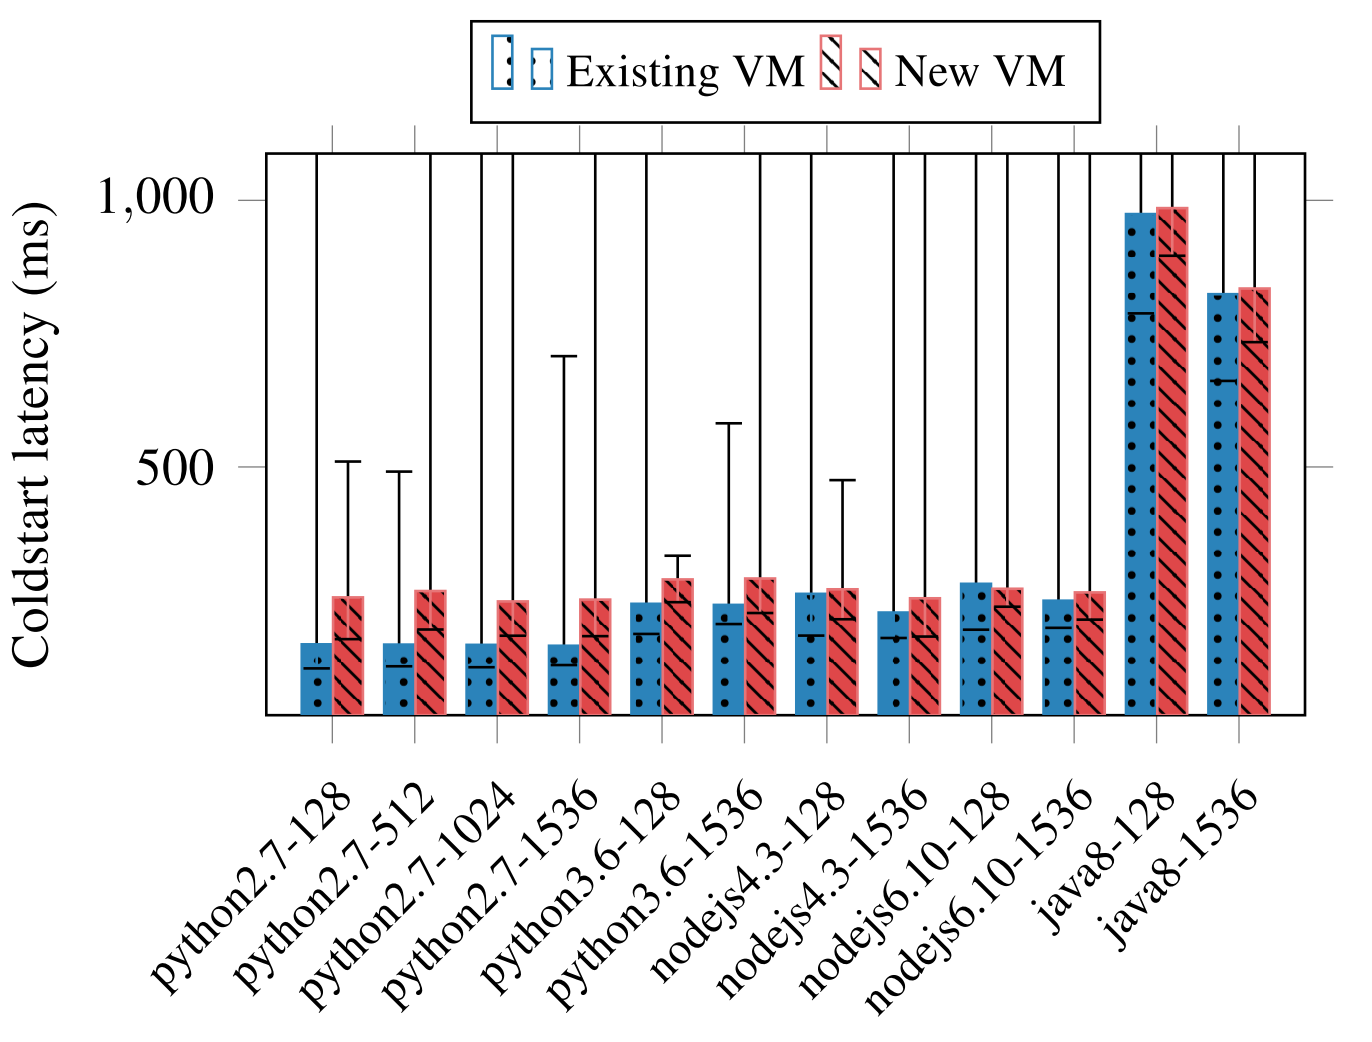
\includegraphics[width=0.5\textwidth]{images/Coldstarts.png}
	\caption{
		Coldstartzeiten von AWS Lambda \autocite[p.~139]{Wang}
	}
	%for reference to this figure
	\label{figure:Coldstarts}
\end{figure}

\subsection{Probleme von Serverless}

\begin{flushleft}
\textbf{Coldstartzeiten:} Jedes Mal wenn eine Funktion nicht mehr gebraucht wird, wird der Container oder die Virtuelle Maschine vom Cloud Provider terminiert und erst beim nächsten Request wieder gestartet. Das führt zu einer längeren Request Zeit, diese zusätzliche Zeit hängt von der Programmiersprache und der Menge an zugewiesenem Speicher ab \autocite[p.~138--139]{Wang}. Abbildung 1 zeigt die verschiedenen Coldstartzeiten von AWS Lambda. Ein Coldstart besteht aus folgenden Abschnitten: \textbf{(1)} Das Starten der Funktion, \textbf{(2)} das Initialisieren der Softwareumgebung der Funktion und \textbf{(3)} die Initialisierung des bereitgestellten Codes. Wobei \textbf{(3)} den größten Einfluss auf die Performance hat.  \autocite[p.~14]{Jonas2019} \break

Das Paper \cite{Wang} beschäftigt sich mit Coldstartzeiten von AWS Lambda. Es wurde herausgefunden, dass es einen Unterschied macht, ob die Virtuelle Maschine beziehungsweiße der Container bereits einmal gestartet wurde oder komplett neu ist, dieser Unterschied ist im Durchschnitt 39 ms. Python hat die niedrigsten Coldstarts (167 – 171 ms) von den getesteten Programmiersprachen. Java hat die höchste Coldstart Latenz (824 – 974ms). Der große Unterschied zwischen den Sprachen könnte damit erklärt werden, dass AWS CPU-Leistung proportional zum Arbeitsspeicher allokiert, das heißt, je mehr Arbeitsspeicher eine Funktion zugewiesen hat, desto mehr Zugriff auf CPU Leistung hat diese, und kann somit Programmierumgebungen schneller starten. Zusätzlich wurde herausgefunden, dass wenn mehrere Funktionen auf einer Virtuellen Maschine gestartet werden, die Coldstart-Latenz auch nach oben geht.

Das Paper \cite{Lloyd} (siehe \textbf{RQ-1}) zeigt, dass der Overhead, der durch das Initialisieren von Dockercontainer entsteht, einen großen Einfluss auf die Performance von Serverless Plattformen hat. Bei diesem Paper ist aber die Methode, wie ermittelt wird, auf welcher VM sich die Funktion befindet, laut \autocite[p.~135 und 137]{Wang} inakkurat.
\break


\textbf{Kompatibilität zwischen Cloud Providern:} Bei Serverless Providern gibt es zurzeit aber noch keine standardisierte Notation wie man eine Funktion definiert \autocite[p.~3]{VanEyk2017}, somit ist nicht gegeben, dass dieselbe Funktion auf einem anderen Cloud Provider funktioniert ohne dessen Programmcode zu ändern. \break


\textbf{Testen:} Tests lokal durchzuführen gestaltet sich in einer Serverless Architektur als schwierig, da die meisten Services der Cloud Provider Closed-Source sind \autocite[p.~3]{VanEyk2017}, diese aber für die Ausführung der Applikation benötigt werden. \break

\end{flushleft}

\begin{figure*}[ht]
	\centering
	\begin{tabular}{r|rrrrrrr}
		                  & $JavaScript$ & $Python$ & $Ruby$ & $Java$ & $Go$ & $C\#$ & $F\#$ \\ \hline
		$AWS\ Lambda$      & $Ja$         & $Ja$     & $Ja$   & $Ja$   & $Ja$ & $Ja$ & $Nein$ \\
		$Azure\ Functions$ & $Ja$         & $Ja$     & $Nein$ & $Ja$   &$Nein$& $Ja$ & $Ja$ \\
		$Google\ Cloud\ Functions$ & $Ja$ & $Ja$ & $Nein$ & $Nein$ & $Ja$ & $Nein$ & $Nein$
	\end{tabular}
	\caption{
		Tabelle der verschiedenen Programmiersprachen der Cloud Provider \autocite[]{faqlambda} \autocite[]{azurefunc} \autocite[]{googlefunc}
	}
	\label{table:ProgrammingLang}
\end{figure*}

\section{WebAssembly}
\label{section:WebAssembly}

WebAssembly ist ein Binary Code Format, das speziell für Browser entwickelt wurde, es erlaubt Low-level Code in Web auszuführen. Laut Spezifikation\footnote{\url{https://webassembly.github.io/spec/core/bikeshed/}} funktioniert WebAssembly aber auch außerhalb von Browsern. WebAssembly ist vor allem der einzige Standard in diesen Bereich, der von allen größeren Browserherstellern unterstützt wird.

\subsection{WebAssembly Vorgänger}

Es gab schon einige Vorgänger von WebAssembly, die versuchten Low-level Code im Browser ausführbar zu machen, die meisten würden jedoch wegen verschiedener Probleme nie in allen Browsern implementiert.

\begin{flushleft}

\textbf{Native Client} \autocite[]{Yee2010} war das erste System, das mittels Sandboxing Maschinen-Code im Web ausführen konnte. Native Client konnte in Google Chrome jedoch nicht so implementiert werden, dass es synchronen Zugriff auf diverse Web- und Javascript-APIs hat \autocite[p.~186]{Haas2017}. Zusätzlich war Native Client oder NaCl nicht portierbar, da es auf einem sehr architekturspezifischen Maschinencode basierte \autocite[p.~186]{Haas2017}. Später wurde dann der Portable Native Client \autocite[]{Donovan2010} entwickelt, der auf LLVM Bytecode basiert um eine bessere Kompatibilität und Portabilität zu erzielen. Es würden jedoch immer noch sehr viele Plattformspezifische Details offengelegt. NaCl und PNaCl wurden lediglich in Google Chrome implementiert \autocite[p.~186]{Haas2017}. 

\hfill \break

\textbf{Emscripten} kompiliert LLVM Bytecode zu einen spezialisierten Subset von JavaScript \autocite[]{Zakai2011}, später zu asm.js\footnote{\url{http://asmjs.org/}} \autocite[p.~186]{Haas2017}. Asm.js ist eine Domainspezifische Sprache, die wie eine statisch typisierte und ähnlich zu Assembler-Sprachen funktioniert \autocite[p.~186]{Haas2017}. Mittlerweile kann LLVM Bytecode mittels Emscripten auch zu WebAssembly Modulen kompiliert werden \autocite[]{Emscripten}.

\end{flushleft}


\subsection{WebAssembly erklärt}

\begin{figure*}[t]
	\centering
	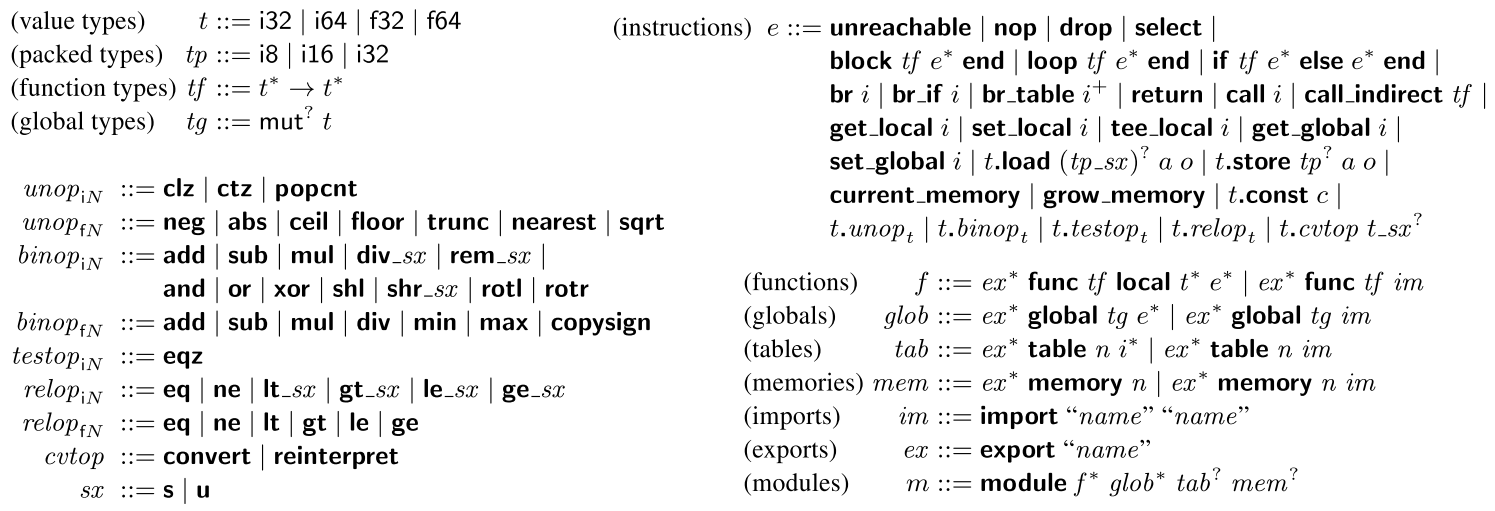
\includegraphics[width=1\textwidth]{images/WebAssemblySyntax.png}
	\caption{
		WebAssembly Syntax \autocite[p.~187]{Haas2017}
	}
	%for reference to this figure
	\label{figure:WASyntax}
\end{figure*}

Da WebAssembly eine neue Technologie ist, werden in diesen Punkt wichtige Grundfunktionalitäten des Standards laut \autocite[p.~186--189]{Haas2017} erklärt. Abbildung 3 zeigt die verschiedenen Komponenten des WebAssembly Byte-Codes.

\begin{flushleft}
\textbf{Module}: Umfassen das gesamte Binary, also ein Modul beinhaltet mehrere Deklarationen von Funktionen, Globals, Tables und Memory. Die Deklarationen eines Modules können unter verschiedenen Namen exportiert oder importiert werden. Eine Instanz eines Modules entspricht einem Programm zusätzlich mit variablen Speicher und einem Executionstack. Das Modul kann dann vom jeweiligen Embedder, zum Beispiel JavaScript importiert werden.

\hfill \break

\textbf{Funktionen}: Eine Funktion nimmt eine beliebige Anzahl an Parametern und gibt welche zurück. Funktionsdeklarationen können nicht inereinander verschachtelt werden. Funktionen können von anderen Funktionen und auch rekursiv aufgerufen werden.

\hfill \break

\textbf{Instruktionen}: Instruktionen sind verschiedene Operationen, die bestimmte Werte und Speicher bearbeiten können, diese werden innerhalb der Funktionen ausgeführt.

\hfill \break

\textbf{Traps}: Falls eine Instruktion einen Fehler verursacht, kann eine Trap ausgelöst werden, die zum sofortigen Abbrechen des Programmes führt. Diese Traps müssen vom jeweiligen Embedder behandelt werden, in JavaScript wird eine Exception mit dem JavaScript und WebAssembly Stacktrace geworfen.

\hfill \break

\textbf{Typen}: WebAssembly Bytecode hat nur 4 verschiedene Basis Variablen Typen, Integer und Floating Point Number, diese in einer 32 und 64bit Version. WebAssembly hat keine Unterscheidung zwischen signed und unsigned Integer, falls es jedoch für die Berechnung wichtig ist kann \_u oder \_s als Suffix hinzugefügt werden.

\hfill \break

\textbf{Lokale Variablen}: Funktionen können lokale Variablen deklarieren, diese könen mittels der \textbf{get\_local} und \textbf{set\_local} Instruktion gesetzt oder gelesen werden.

\hfill \break

\textbf{Globale Variablen}: Es können auch Variablen global in einem Modul deklariert werden, diese können dann in mehreren Funktionen verwendet werden.

\hfill \break

\textbf{Memory Managment:} In WebAssembly werden alle Variablen und Werte in einem Array von Bytes gespeichert, diesen Array bezeichnet man als Memory oder linear Memory. Ein Modul hat jeweils einen Memory Array, dieser wird mit einer bestimmten Größe initialisiert, kann aber im Laufe des Programmes dynamisch erweitert werden. Falls es zu einem Out-of-Memory Fehler kommt gibt die Instruktion \textbf{grow\_memory}, die verwendet wird, um den Speicher dynamisch zu erweitern, den Wert -1 zurück. Der Speicher wird immer um 64KiB erweitert. 
Die Adresse die zusätzlich zu anderen Parametern (\textit{a}\footnote{static alignment exponent \autocite[p.~188]{Haas2017}}, \textit{o}\footnote{positive static offset \autocite[p.~188]{Haas2017}} und \textit{tp}\footnote{optional static width \autocite[p.~188]{Haas2017}} ) benötigt wird, um auf den Speicher mittels \textbf{load} zuzugreifen, ist ein unsigned 32 bit Integer, der bei 0 startet. Es können immer 8, 16, 32 und 64bit aus dem Speicher geladen werden. Der Lineare Speicher ist komplett vom Code-Space und Executionstack getrennt, das heißt, dass ein fehlerhaftes WebAssembly Programm nicht seine Laufzeitumgebung verändern kann, ein fehlerhaftes Programm kann nur dessen eigenen Speicher manipulieren. Dadurch, dass der Speicher so isoliert ist, können auch nicht vertrauenswürdige WebAssembly Module ausgeführt werden. \break

\textbf{Syntax} Die meisten Assembler Sprachen springen meistens von Instruktion zu Instruktion, WebAssembly hingegen verhält sich wie eine Programmiersprache. WebAssembly implementiert einen sogenannten Structured Control Flow. WebAssembly kann somit besser die Validität des Programmes feststellen, zusätzlich kann jedes Modul in einen Durchgang validiert und kompiliert werden.
Manche Sprachen Konstrukte müssen mit \textbf{end} geschlossen werden, zum Beispiel \textbf{block}, \textbf{if} und \textbf{loop}.

\end{flushleft}

\subsection{Ziele von WebAssembly}

WebAssembly versucht gleichzeitig das Beste seiner Vorgänger zu verwenden, aber vor allem ist das Ziel, deren Probleme zu lösen.

\begin{flushleft}


\textbf{Sicherheit}: Sicherheit ist ein großer Faktor im Web, da sehr viel Programm-Code aus nicht vertrauenswürdigen Quellen stammt. Eine Low-Level Sprache im Web muss vor allem unabhängig von der Umgebung, in der sie ausgeführt wurde, laufen, um Memory Leaks und dergleichen zu verhindern \autocite[p.~185-186]{Haas2017}. Jedes Modul hat seinen eigenen Arbeitsspeicher, der auch unabhängig von der Host-Umgebung ist. Ein WebAssembly Modul kann somit nicht seine Umgebung, in der es ausgeführt wurde, beeinflussen \autocite[p.~188]{Haas2017}. Das Paper von \cite{Lehmann} zeigt jedoch wie Attacken die auf Nativen Plattformen wie x86 schon länger nicht mehr möglich sind, auf WebAssembly wieder funktionieren.

\hfill \break

\textbf{Performance}: Ein Nativer Maschinencode, der entweder von Hand geschrieben oder durch einen Compiler optimiert wurde, kann die volle Leistung einer Maschine ausnützen \autocite[p.~186]{Haas2017}. WebAssembly ist im Vergleich to Nativen Maschinencode (x86) im Durchschnitt 1,55 mal in Chrome und 1,45 mal in Firefox langsamer \autocite[p.~118]{Jangda}.

\hfill \break

\textbf{Portable}: Im Web werden verschiedenste Geräte verwendet. Ein Low-Level Bytecode sollte auf jeder Architektur laufen, er sollte auch in jeden Browser implementiert werden. Um das zu erreichen, muss dieser unabhängig von Betriebssystem, Browser und Hardware sein. \autocite[p.~186]{Haas2017}

\hfill \break

\textbf{Kompakt}: Da dieser Low-Level Code über das Netzwerk ausgeliefert wird, sollte er so kompakt wie möglich sein, um Bandbreite zu sparen. \autocite[p.~186]{Haas2017}

\end{flushleft}

\begin{figure}[t]
	\centering
	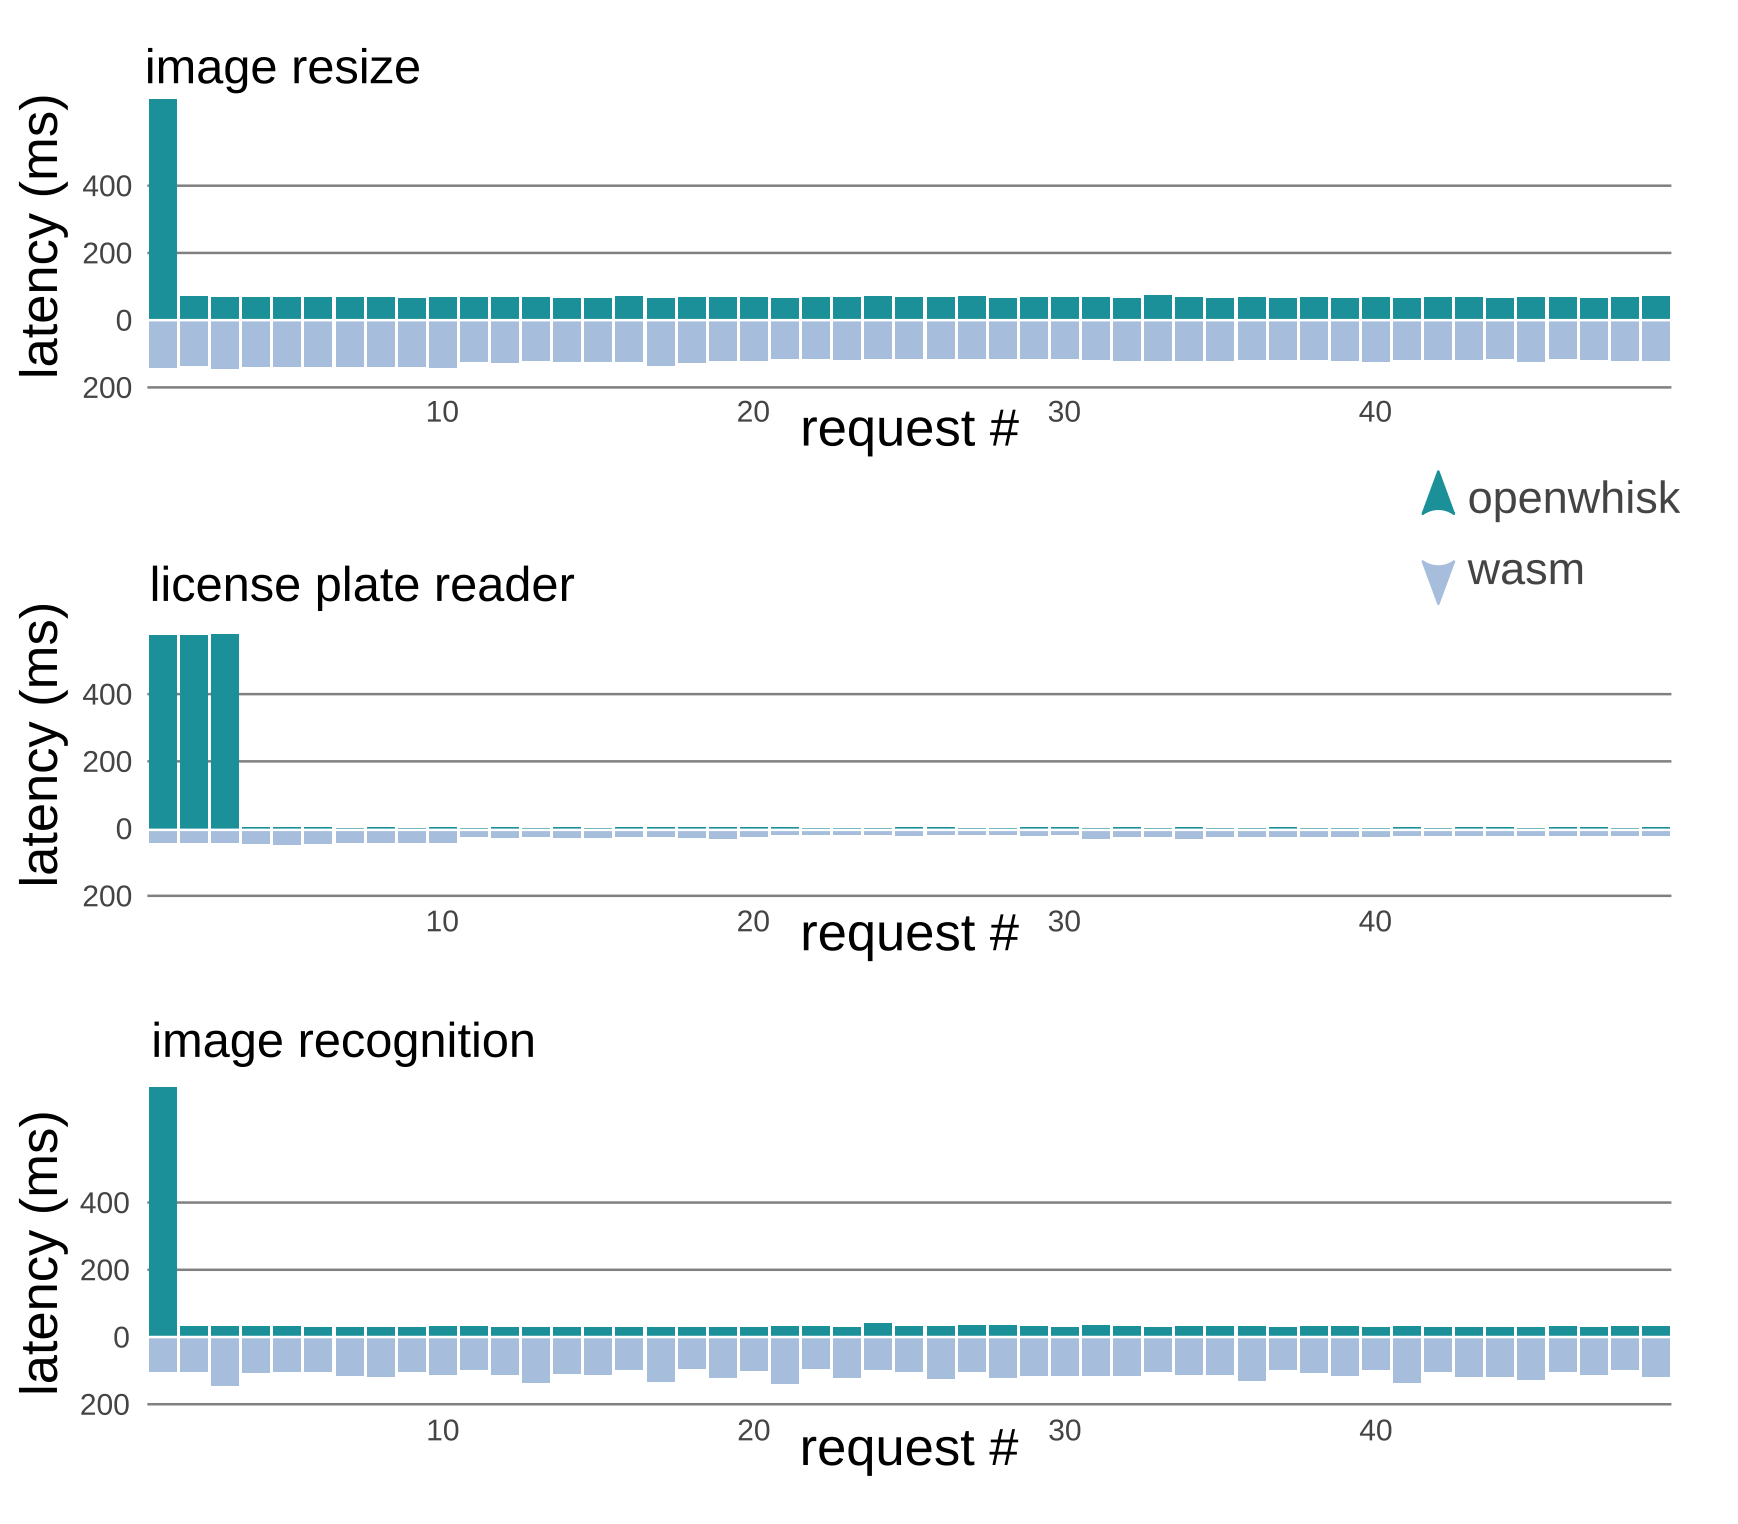
\includegraphics[width=0.5\textwidth]{images/RequestTimesSlow.png}
	\caption{
		Startup Latenzen OpenWhisk vs. WebAssembly \autocite[p.~232]{Hall2019}
	}
	%for reference to this figure
	\label{figure:StartupLatFirst}
\end{figure}

\begin{figure}[t]
	\centering
	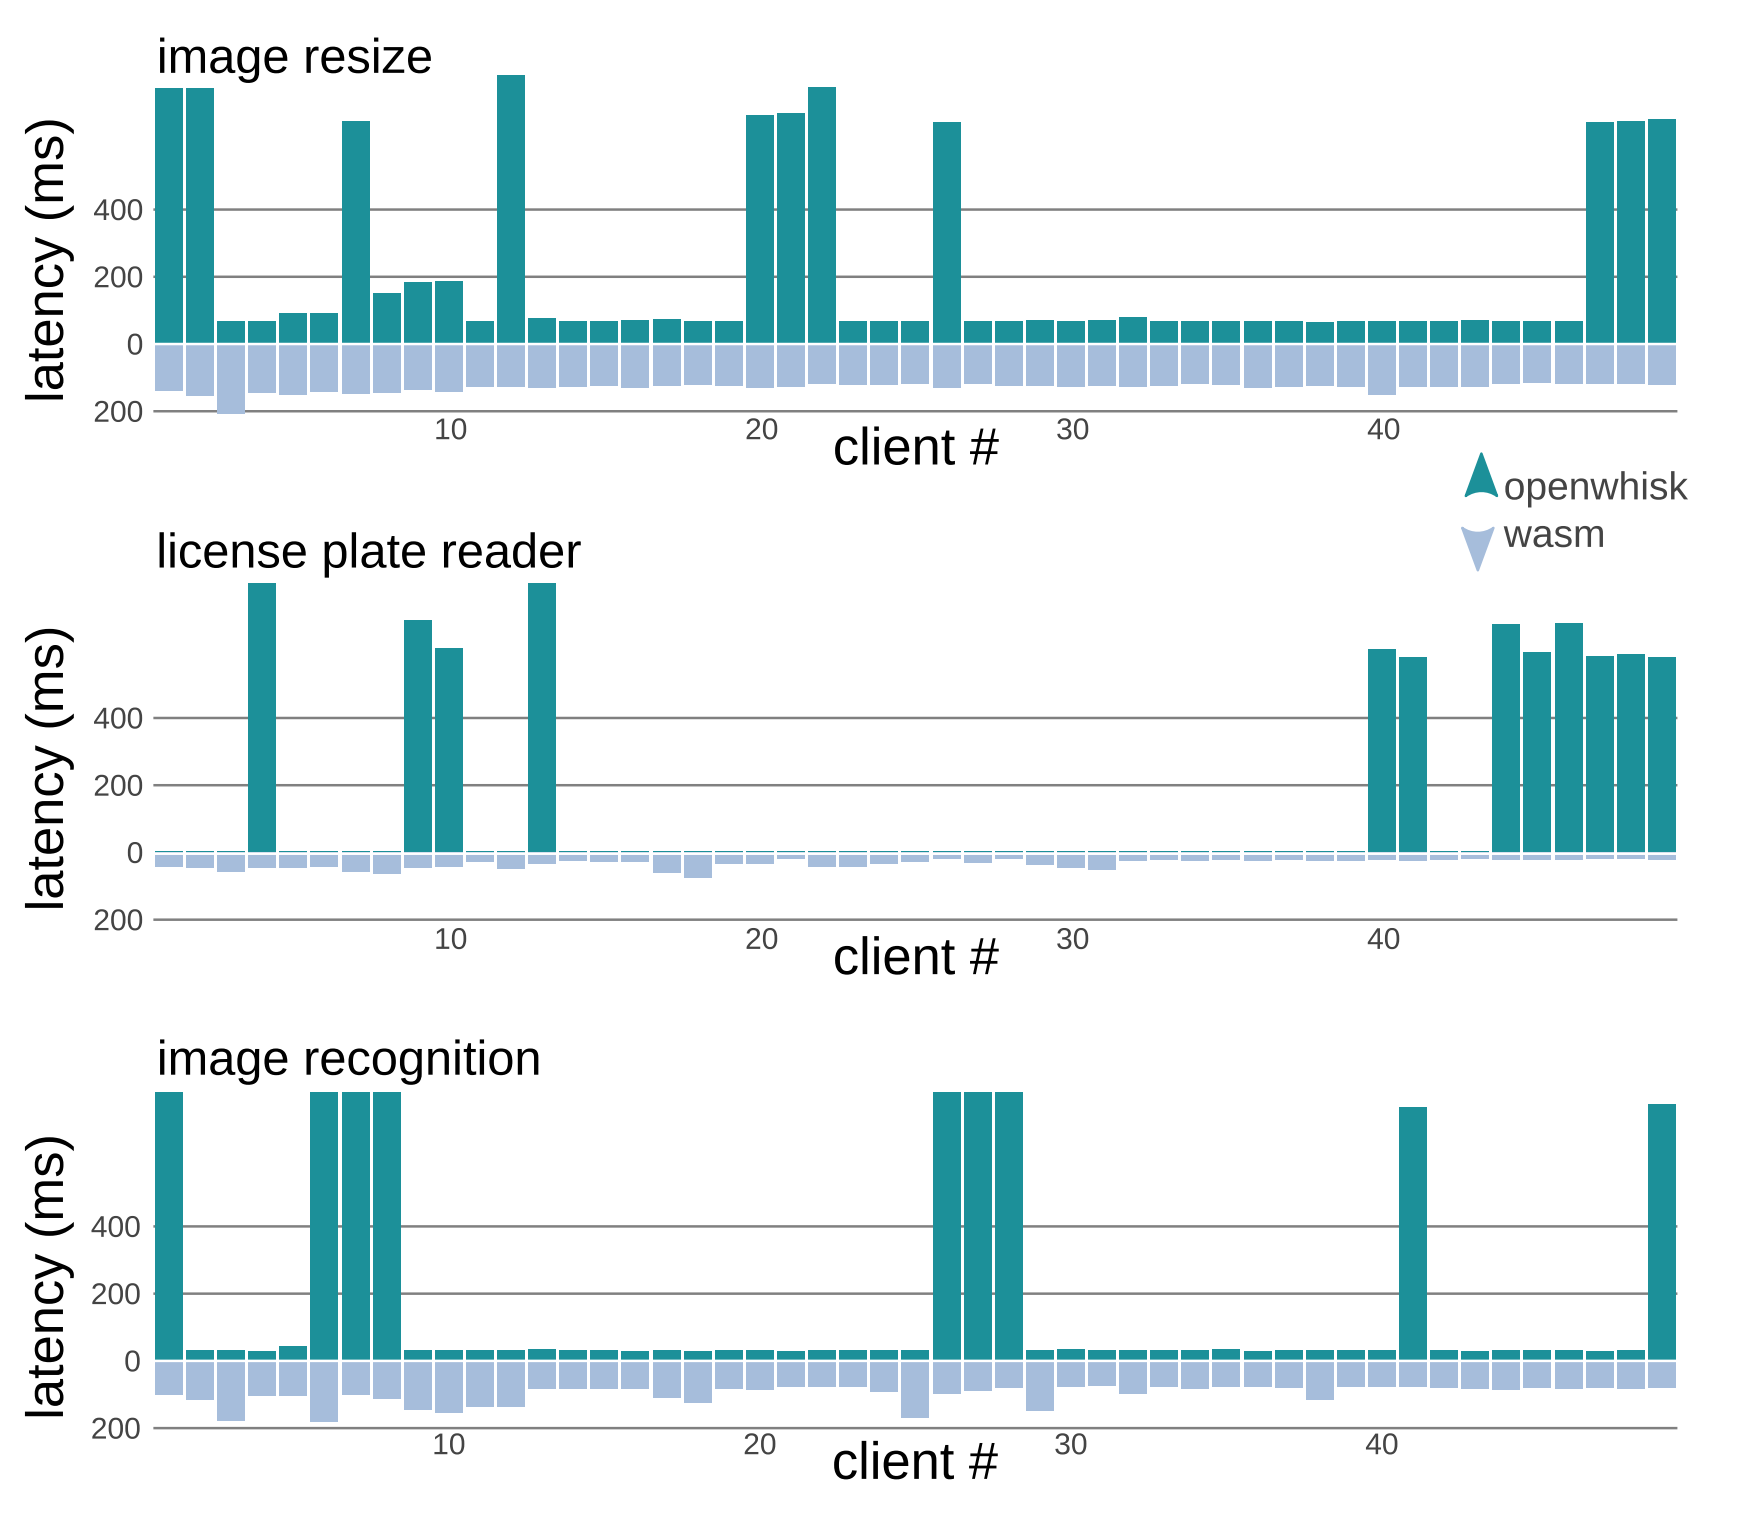
\includegraphics[width=0.5\textwidth]{images/RequestTimesReal.png}
	\caption{
		Startup Latenzen OpenWhisk vs. WebAssembly \autocite[p.~233]{Hall2019}
	}
	%for reference to this figure
	\label{figure:StartupLatSecond}
\end{figure}

\section{Serverless mit WebAssembly}
\label{section:Serverless mit WebAssembly}

Serverless hat noch einige Probleme, diese wurden im Punkt \textit{2.3 Probleme von Serverless} in dieser Arbeit genau erläutert. WebAssembly hat einige Eigenschaften, die zur Lösung dieser Probleme beitragen könnten, und mehrere Firmen und Arbeiten beschäftigen sich bereits mit dieser Thematik. Das Paper von \cite{Hall2019} zeigt vor allem wie eine auf WebAssembly basierende Serverless-Plattform die gleiche Isolation und fast die gleiche Performance wie eine Container-basierte Plattform erreichen kann. Zusätzlich wird gezeigt, dass durch das Verwenden von WebAssembly die Coldstartzeit reduziert werden kann. 

\subsection{Coldstarts}

Die durchschnittliche Coldstartzeit von Serverless-Funktionen ist von Provider zu Provider und von Programmiersprache zu Programmiersprache unterschiedlich siehe Punkt \textit{2.3 Probleme von Serverless}. Die WebAssembly Spezifikation\footnote{\url{https://webassembly.github.io/spec/core/bikeshed/}} erwähnt nicht explizit den Browser als Embedder von WebAssembly, es kann auch WebAssembly außerhalb des Browsers ausgeführt werden.

In diesem Paper \cite{Hall2019} werden herkömmliche Serverless Funktionen, also mit Docker Container, mit einer Lösung die WebAssembly Module verwendet, verglichen. Als Serverless-Backend wurde OpenWhisk \footnote{\url{https://openwhisk.apache.org/}} verwendet. Auf die Ergebnisse der Container-basierten Lösung verweise ich auf \textit{OpenWhisk} und bei den Ergebnissen von der WebAssembly-basierenden Lösung verweise ich auf \textit{Wasm}. Hier fällt auf das \textit{OpenWhisk} bei einem Warmstart um 1.5 - 3x schneller ist als \textit{Wasm}. Jedoch ist bei \textit{OpenWhisk} der erste Request (Coldstart) um einiges langsamer. Diese Coldstarts passieren bei einem realistischen Workload jedoch viel öfter, in Abbildung 4 wurde mit einem einzelnen Gerät mehrere Funktionsaufrufe hintereinander durchführt, hier ist im Durchschnitt \textit{OpenWhisk} schneller. In Abbildung 5 wurde ein realistischerer Workload (Multiple Client, Multiple Access Workload, d.h. mehrere Geräte greifen öfter auf die gleiche Ressource zu) verwendet, und hier sieht man, dass \textit{Wasm} im Durchschnitt schneller ist. \textit{Wasm} verhält sich viel berechenbarer als \textit{OpenWhisk}. Dieses Paper wurde im Kontext von IoT\footnote{Internet of Things} Geräten geschrieben, um herauszufinden, ob mehr Requests pro Sekunde mit \textit{Wasm} oder mit \textit{OpenWhisk} abgearbeitet werden können.



\subsection{Programmiersprachen unabhängig}

Eines der Probleme von Serverless war, dass man oft von Cloud Providern abhängig ist, und auch deren Programmiersprachen wählen muss, denn diese Provider bieten nicht alle Programmiersprachen an (siehe Abbildung 2). Dieses Problem der Programmiersprachen-Abhängigkeit könnte auch mittels WebAssembly gelöst werden. Projekte wie Emscripten\footnote{\url{https://emscripten.org/}} oder wasm-pack\footnote{\url{https://github.com/rustwasm/wasm-pack}} ermöglichen es zum Beispiel LLVM Bytecode oder Rust zu WebAssembly zu kompilieren. Jeder Cloud Provider unterstützt WebAssembly Module, da es in den neueren Versionen von NodeJS implementiert ist \autocite[]{Wasm}, das erlaubt es WebAssembly Module in JavaScript zu importieren. Somit muss man nur den Code aus einer Programmiersprache, die zu WebAssembly kompiliert werden kann, zu einem Modul kompilieren und man könnte dieses dann in NodeJS importieren und verwenden. Das Paper \cite{Letz2018} zeigt wie der Compiler der Faust DSP Audio Programmiersprache zu WebAssembly kompiliert und im Browser verwendet werden kann.

\section{Fazit}

Meiner Erfahrung nach kann das verwenden von Serverless Funktionen einiges an Arbeit verringern. Es ist jedoch um einiges komplizierter zu Lernen und viel abstrakter, und oft ist es einfacher einen Virtuellen Server zu verwenden. Zusätzlich dazu gibt es zurzeit viele Frameworks wie Symfony, Ruby on Rails oder Laravel, die viel erleichtern, mit Serverless muss man diese Dienste entweder als Service von einem Cloud Provider hinzufügen oder selbst implementieren. Serverless ist meiner Meinung nach im Großen und Ganzen eine gute Ergänzung für die derzeitige Serverlandschaft, und vor allem für kleine Projekte und Projekte mit schwankender Auslastung, ist Serverless sehr gut geeignet, da Provider meist ein flexibleres Preismodell für Serverless anbieten als für klassiche VM Instanzen. Das größte Problem von Serverless ist in meinen Augen zurzeit die fehlende Kompatibilität (siehe Punkt \textit{2.3 Probleme von Serverless}) zwischen den jeweiligen Cloud Providern, denn wenn man sich für einen Provider entscheidet, ist es später schwierig die komplette Applikation umzuziehen.

Durch WebAssembly gibt es jetzt einen Low-Level Bytecode, der in einem Browser in einer isolierten Sandbox ausgeführt werden kann, und die oben genannten Kriterien erfüllt (siehe Punkt \textit{3.3 Ziele von WebAssembly}). Das wichtigste Feature ist die Plattform Unabhängigkeit, die es ermöglicht WebAssembly überall auszuführen. Zusätzlich kann jede Programmiersprache in ein WebAssembly Modul kompiliert werden, somit kann man Software-Bibliotheken, die in JavaScript schlechter, beziehungsweise nicht implementiert wurden, einfach zu einem WebAssembly Modul kompilieren und im Browser verwenden.

Wenn man WebAssembly mit Serverless kombiniert können einige Probleme von Serverless gelöst werden (siehe Punkt \textit{4.1 Coldstarts} und \textit{4.2 Programmiersprachen unabhängig}). \cite{Hall2019} zeigen zwar, dass Serverless Plattformen die auf Container oder Virtuellen Maschinen basieren bei Warmstarts schneller sind als WebAssembly Module, jedoch haben sie eine hohe Coldstart-Latenz, und da in einer realen Anwendung öfter Coldstarts vorkommen wäre WebAssembly hier berechenbarer und im Durchschnitt schneller.